%%%%%%%%%%%%%%%%%%%%%%%%%%%%%%%%%%%%%%%%%%%%%%%%%%%%%%%%%%%%%%%%%%%%%%%%%%%%%%%

\chapter{DESENVOLVIMENTO}

Nesta seção, são apresentados os procedimentos e etapas realizados para a execução do projeto. Inicialmente, descrevem-se os materiais e métodos adotados, seguidos pelos processos de implementação, oficinas e estratégias de avaliação utilizadas no CPTECRAFT.

\section{Material e Métodos}

Para a execução do projeto CPTECRAFT, foram utilizados recursos tecnológicos e materiais de baixo custo, com o propósito de criar um ambiente imersivo e educativo, fundamentado na construção de uma réplica virtual do CPTEC/INPE no jogo Minecraft. Inicialmente, adotou-se a versão Minecraft Java Edition, desenvolvida em linguagem de programação Java, como base para a criação do espaço virtual. Essa escolha possibilitou a utilização da plataforma Forge, ferramenta essencial para instalação de modificações, permitindo a inserção de recursos avançados que aproximam a experiência digital da estrutura real do CPTEC/INPE.

A metodologia do projeto foi estruturada em três etapas principais, planejadas para garantir que o CPTECRAFT alcance seu objetivo de despertar o interesse dos jovens pela ciência e tecnologia de forma acessível e envolvente:

\subsection{Desenvolvimento do Ambiente Virtual}

Nessa fase, foi realizada a construção da réplica virtual do CPTEC/INPE no Minecraft, utilizando a plataforma Forge e modificações que possibilitam maior proximidade ao ambiente real. Para assegurar a coerência científica da representação, foram utilizadas imagens e plantas do centro, além da colaboração de pesquisadores do CPTEC/INPE.

\subsection{Implementação da Realidade Virtual}

A segunda etapa consistiu na integração da tecnologia de Realidade Virtual (VR) por meio da modificação Vivecraft, permitindo uma experiência imersiva em perspectiva de primeira pessoa. Paralelamente, foi desenvolvido um modelo de óculos VR artesanal e de baixo custo, utilizando materiais recicláveis como papelão, elásticos e lentes plásticas. Essa iniciativa buscou garantir acessibilidade e democratização do acesso à tecnologia.

\subsection{Oficinas Educativas com Gamificação}

A terceira etapa do projeto, que prevê a realização de oficinas educativas voltadas para crianças e adolescentes, será retomada durante a próxima vigência da bolsa de iniciação científica. Nessas oficinas, os participantes aprenderão sobre realidade virtual, a construção dos óculos VR e a exploração científica dentro do ambiente do CPTECRAFT. A proposta adota uma metodologia baseada em gamificação, utilizando desafios interativos, missões e elementos lúdicos para aumentar o engajamento e promover a aprendizagem ativa.

Embora o projeto já tenha sido apresentado em eventos e feiras científicas — nos quais visitantes puderam interagir com a réplica virtual, testar óculos VR e participar das dinâmicas propostas — a realização das oficinas planejadas especificamente para o público-alvo do projeto ainda está por acontecer. Após sua implementação, serão coletados feedbacks qualitativos e quantitativos dos participantes, que servirão para mensurar os resultados alcançados e orientar futuras aplicações e aprimoramentos do CPTECRAFT.

\section{Resultados}

Nesta seção, apresentamos a análise dos dados obtidos a partir da implementação do projeto CPTECRAFT, que envolveu a construção da réplica virtual do CPTEC/INPE, a integração da realidade virtual, o desenvolvimento dos óculos VR de baixo custo e a aplicação das oficinas gamificadas, além da avaliação do impacto junto aos participantes.

\subsection{Construção da réplica virtual}

A réplica virtual do CPTEC/INPE foi desenvolvida com alta fidelidade arquitetônica e funcional, possibilitando a exploração interativa dos principais espaços da instituição. Foram reproduzidas áreas como laboratórios meteorológicos, setores administrativos e espaços de divulgação científica. A plataforma Forge permitiu a personalização do ambiente com texturas específicas e placas informativas, proporcionando um contexto educativo coerente e envolvente.

\begin{figure}[H]
    \centering
    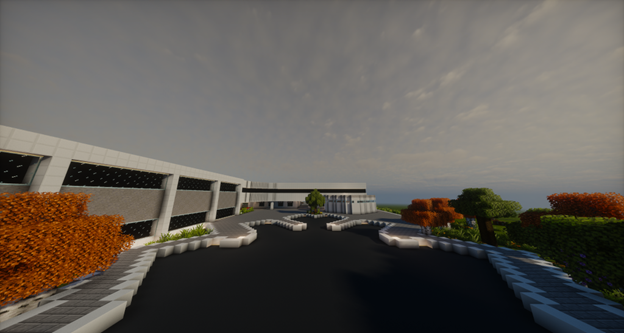
\includegraphics[width=0.9\textwidth]{docs/figuras/Imagem1.png}
    \caption{Réplica virtual do CPTEC/INPE construída no Minecraft.}
    \label{fig:replica_cptec}
\end{figure}

\subsection{Implementação da Realidade Virtual}

A integração do mod Vivecraft permitiu que os participantes explorassem o ambiente virtual em primeira pessoa, aumentando a sensação de imersão no espaço virtual do CPTEC. Essa experiência ampliou o engajamento e facilitou a compreensão dos conceitos científicos incorporados nas missões que compõem a gamificação do ambiente.

\subsection{Desenvolvimento e utilização dos óculos VR artesanais}

O projeto desenvolveu um modelo acessível de óculos de realidade virtual confeccionados com materiais recicláveis, como papelão, elásticos e lentes plásticas reaproveitadas. Este design visa estimular a criatividade, incentivar práticas sustentáveis e ampliar a inclusão tecnológica entre os jovens participantes. Materiais e etapas de montagem foram cuidadosamente planejados e documentados para facilitar sua replicação futura, incluindo a criação de manuais ilustrados.


\begin{figure}[H]
    \centering
    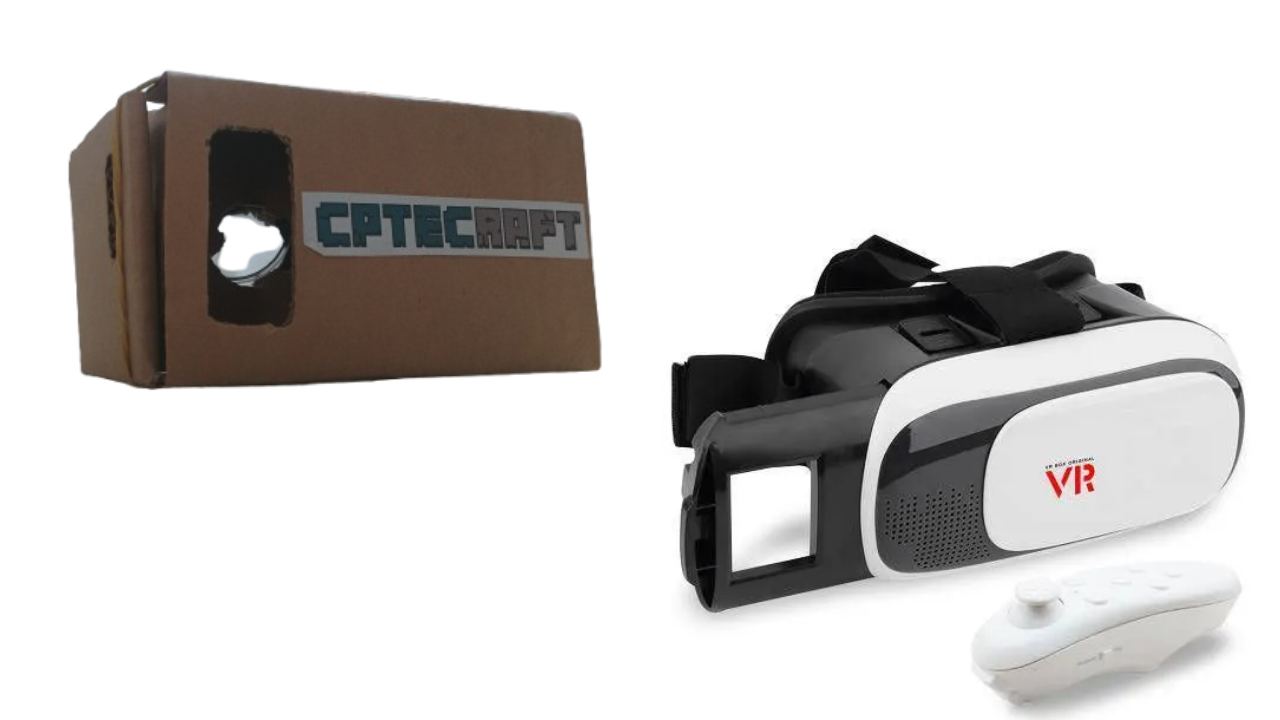
\includegraphics[width=0.5\textwidth]{docs/figuras/Imagem2.png}
    \caption{Óculos VR confeccionados artesanalmente com materiais recicláveis.}
    \label{fig:oculos_vr}
\end{figure}

A implementação prática da confecção destes óculos será realizada nas oficinas educativas previstas para a próxima etapa do projeto, ocasião em que os jovens poderão ser guiados na montagem dos dispositivos, promovendo uma experiência prática e interdisciplinar.

\subsection{Gamificação aplicada ao ensino}

As atividades planejadas envolvem missões e desafios gamificados que exigem aplicação de conceitos de meteorologia, engenharia e sustentabilidade para avançar em objetivos virtuais dentro do ambiente CPTECRAFT. Essa metodologia visa aumentar o engajamento e a motivação pelo aprendizado, associando a interatividade e a diversão a temas científicos relevantes.

Essas oficinas e dinâmicas ainda estão por ser implementadas. Após sua realização, espera-se coletar relatos e avaliações dos participantes para aperfeiçoamento contínuo da proposta pedagógica.

\subsection{Eventos científicos e recepção do público}

No III Encontro de Jovens Cientistas, o CPTECRAFT foi apresentado a crianças, adolescentes e educadores, que interagiram com o ambiente virtual, construíram os óculos VR e participaram das dinâmicas. A receptividade foi muito positiva, demonstrando o potencial da iniciativa para ampliações futuras.

\begin{figure}[H]
    \centering
    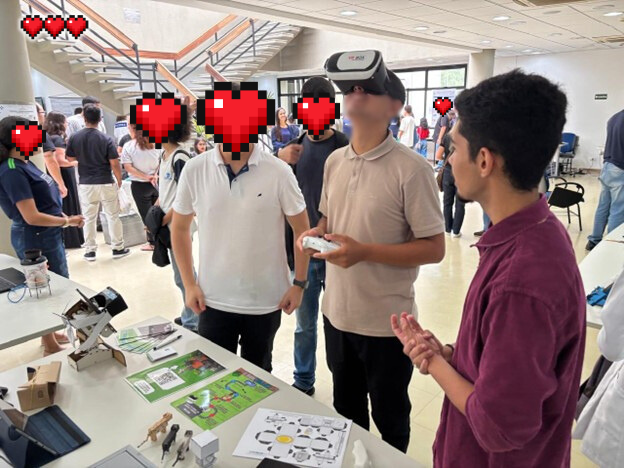
\includegraphics[width=0.6\textwidth]{docs/figuras/Imagem3.png}
    \caption{Participantes interagindo durante o III Encontro de Jovens Cientistas.}
    \label{fig:evento_joes}
\end{figure}

\subsection{Análise quantitativa e qualitativa dos feedbacks}

Para avaliar o impacto do projeto, foi aplicado um questionário utilizando escala Likert de 1 a 5. A Tabela 2.1 mostra os resultados quantitativos das respostas principais.

\begin{table}[!ht]%[htbp] % opções de colocação da tabela no texto
  \begin{center}% use sempre um ambiente para as tabelas
% (opções: center (recomendado), flushright, flushleft)
% NÃO USE \centering com TABELAS se houver \FONTE!
  \caption{Resultados do Questionário (escala de 1 a 5)}
    \begin{tabular}{l|c|c}
\hline % desenha uma linha horizontal
Questão & Média & Desvio Padrão \\
\hline % desenha uma linha horizontal
Motivação para aprender ciência aumentou? & 4,6 & 0,5 \\
Facilidade de uso dos óculos VR? & 4,1 & 0,6 \\
Diversão/engajamento nas atividades? & 4,8 & 0,4 \\
Recomendaria para outros alunos? & 4,7 & 0,5 \\
\hline % desenha uma linha horizontal
    \end{tabular}
  \end{center}
  \FONTE{Dados coletados durante III Encontro de Jovens Cientistas.}
\end{table}

Esses dados indicam alto nível de satisfação e engajamento dos participantes. Comentários espontâneos corroboram as avaliações quantitativas, destacando a experiência prática e o uso da realidade virtual como aspectos muito valorizados:

\begin{itemize}
    \item “Achei muito interessante a possibilidade de poder explorar o CPTEC no Minecraft.”  
    \item “O CPTECRAFT já está disponível ao público?.”  
    \item “Queremos ficar atualizado com os avanços do projeto.”  
\end{itemize}

Em síntese, os resultados quantitativos e qualitativos confirmam a eficácia da metodologia empregada, evidenciando uma aceitação positiva e um alto grau de motivação entre as crianças e adolescentes participantes, consolidando o CPTECRAFT como uma ferramenta promissora para a popularização da ciência e inovação pedagógica.


\section{Discussão dos Resultados}

Os resultados obtidos confirmam a alta aceitação do público e o engajamento gerado pela proposta. Entre os pontos mais valorizados pelos participantes destaca-se a integração entre ciência e jogos digitais, a possibilidade de experiências imersivas com óculos VR de baixo custo e a abordagem gamificada, que transforma conteúdos complexos em desafios interativos e atrativos.

As sugestões coletadas, como a ampliação do acesso a diferentes plataformas, a inserção de jogos educativos e o fortalecimento da divulgação em redes sociais, indicam oportunidades de expansão e melhoria contínua. Essas recomendações reforçam a importância de consolidar o CPTECRAFT como um recurso pedagógico escalável, adaptável a múltiplos contextos escolares e capaz de integrar inovação tecnológica com práticas educativas.

\chapter{Resultados Esperados}

A continuidade do projeto CPTECRAFT espera alcançar resultados expressivos como:  

\begin{itemize}
  \item Ampliar o engajamento de crianças e adolescentes nas áreas STEM por meio de experiências interativas e acessíveis;  
  \item Expandir a utilização da plataforma em escolas públicas e eventos científicos, democratizando o acesso ao ensino inovador;  
  \item Capacitar professores para integrá-lo em suas práticas pedagógicas, promovendo uma formação continuada;  
  \item Desenvolver materiais didáticos e manuais que facilitem a replicação do projeto em diferentes contextos;  
  \item Aperfeiçoar os instrumentos avaliativos para realizar monitoramento constante do impacto educacional;  
  \item Fortalecer parcerias institucionais e captar recursos para assegurar a sustentabilidade e expansão da iniciativa.  
\end{itemize}